\chapter{Particle Size Distribution Estimation in Supersonic PIV Experiments}\label{ch:fsu_data}

The particle tracking code developed in Chapter \ref{ch:lpt} is utilized to create a new methodology to understand the particle size distribution during a PIV experiment in shock-laden flows. This is extended to a shock interaction experiment conducted at Florida State University (FSU).

\section{Introduction}

Non-intrusive optical velocimetry techniques, such as Particle Image Velocimetry (PIV), have become indispensable tools for investigating flow fields, particularly in the design and analysis of aerospace systems. These techniques employ tracer particles illuminated by laser sheets, with high-speed cameras capturing their motion to reconstruct velocity fields through advanced cross-correlation algorithms. For accurate flow characterization, it is crucial that the tracer particles closely follow the flow field. However, numerous studies (e.g., Samimy et al. \cite{samimy1991}, Melling \cite{melling1997}, Koike et al. \cite{koike2007}, Burns et al. \cite{burns2015}, Kalagotla et al. \cite{kalagotla2018, kalagotla2020}) have demonstrated that, in complex supersonic flow fields, particle inertia often limits the effectiveness of tracer particles, introducing significant measurement uncertainty.

The increasing adoption of PIV, particularly for analyzing large flow fields in supersonic regimes, underscores the importance of careful tracer particle selection. Optimal particle selection balances tracking fidelity, ease of use, and cost. Experimenters typically rely on nominal particle specifications provided by manufacturers or the distribution obtained from their seeder to report the particle size distribution for uncertainty quantification. However, these specifications often fail to represent the true particle characteristics in experimental conditions due to agglomeration, breakup, and measurement limitations, including the PIV camera’s sensitivity to light scattering (Urban and Mungal \cite{urban2001}, Mitchell et al. \cite{mitchell2011}, Williams et al. \cite{williams2015}).

Particle response analysis, a standard method to evaluate particle tracking capability, determines the response time of particles to flow changes. In a response analysis, the PIV measurements study an oblique shock similar to the conditions of the actual study. The velocity field obtained is used to measure the relaxation distance, which can be used to estimate the response time from which mean particle size can be inferred. This response time quantifies the uncertainty introduced by particles in PIV measurements. It is often represented by the dimensionless Stokes number ($S_t$), defined as the ratio of the particle relaxation time to the characteristic time scale of the flow. A Stokes number significantly less than one indicates good particle tracking, whereas higher values suggest poor tracking performance (Samimy et al. \cite{samimy1991}). The flow time scale depends on the characteristic length of interest in a given study. This could range from a geometric length when studying flow interactions with a solid body to the thickness of a shock wave if that is of focus. This factor needs to be carefully determined based on the scope of a given experiment.\par

Estimating the effective particle properties, such as size and density, requires a detailed analysis of particle dynamics, often using empirical drag models. Traditional models like Stokes drag may not adequately capture the inertial, compressibility, and rarefaction effects that dominate in supersonic flows. More sophisticated models, such as those by Tedeschi et al. \cite{tedeschi1999} and Loth \cite{loth2008}, have been developed to address these complexities. A recent work by Kalagotla et al. \cite{kalagotla2024} demonstrated that the particle dynamic history (PDH), which accounts for a particle’s interaction with a series of flow features, plays a significant role in PIV measurement uncertainties. This highlights the need for precise particle response analysis to quantify uncertainties and improve measurement reliability. Traditionally, particle response has been studied by analyzing particle velocity across an oblique shock, allowing the estimation of mean particle size by considering the material density. Williams et al. \cite{williams2015} proposed a two-oblique-shock analysis to solve for nominal particle size and density uniquely, addressing limitations in traditional single-shock methods.\par

Building on this foundation, this study introduces a novel methodology to estimate particle size distributions directly from PIV data. The approach involves isolating particle response data from oblique shock experiments and applying exponential decay analysis, assuming particles are spherical to reconstruct the underlying size distribution. Due to its nature, this could be expanded to any supersonic experiments with an oblique shock, potentially removing the need for a separate particle response study setup. The methodology is extended to the experimental data from the Polysonic Wind Tunnel at Florida State University, which features Mach 2 flows with varying shock interaction configurations. This work highlights the role of spatial resolution and interrogation window size in determining the Stokes number and provides insights into particle dynamics in supersonic PIV experiments.

This methodology aims to enhance the accuracy of particle response studies, which are essential for quantifying uncertainties related to particle dynamics in PIV. Improving the reliability of PIV measurements in complex flow environments enables a more comprehensive understanding of particle size distributions and Stokes numbers as functions of spatial resolution. This advancement significantly enhances our ability to address uncertainties associated with particle inertia bias in particle image velocimetry (PIV) experiments.\par

\section{Shock interaction experimental setup}
This section presents the setup and background of the high-speed wind tunnel tests conducted at Florida State University, which provided experimental data for particle lag and sizing in the present study. First, the wind tunnel and its operating conditions are detailed, followed by the test geometry and PIV setup. Finally, the PIV seeding setup is presented.

\subsection{Polysonic Wind Tunnel}
The Polysonic Wind Tunnel at Florida State University is a blowdown wind tunnel capable of operating over the Mach number range of 0.2 to 5. Its test section has a cross-section of 0.305 x 0.305 m. In the supersonic regime employed in the current study, fixed nozzle blocks are used for Mach 2, 3, and 4, along with a solid wall test section, as shown in Fig. \ref{fig:PSWT}, to ensure high flow quality and optical access from four sides. The tunnel was supplied with 150 m\textsuperscript{3} air stored at 3.5 MPa, providing run times of approximately 60 s depending on test conditions. The tunnel was not actively heated for the present tests, and the air was maintained at a near-ambient stagnation temperature throughout the run, as monitored by a Resistance Temperature Detector (RTD) mounted in the tunnel's stagnation chamber. Stagnation and static pressures are monitored throughout the run by Baratron pressure transducers. The tunnel stagnation pressure is actively controlled during each run-through adjustment of the tunnel control valve, maintaining stagnation pressures of 0.28, 0.45, and 1.17 MPa at Mach 2, 3, and 4, respectively. 

\begin{figure}[ht!]
    \centering
    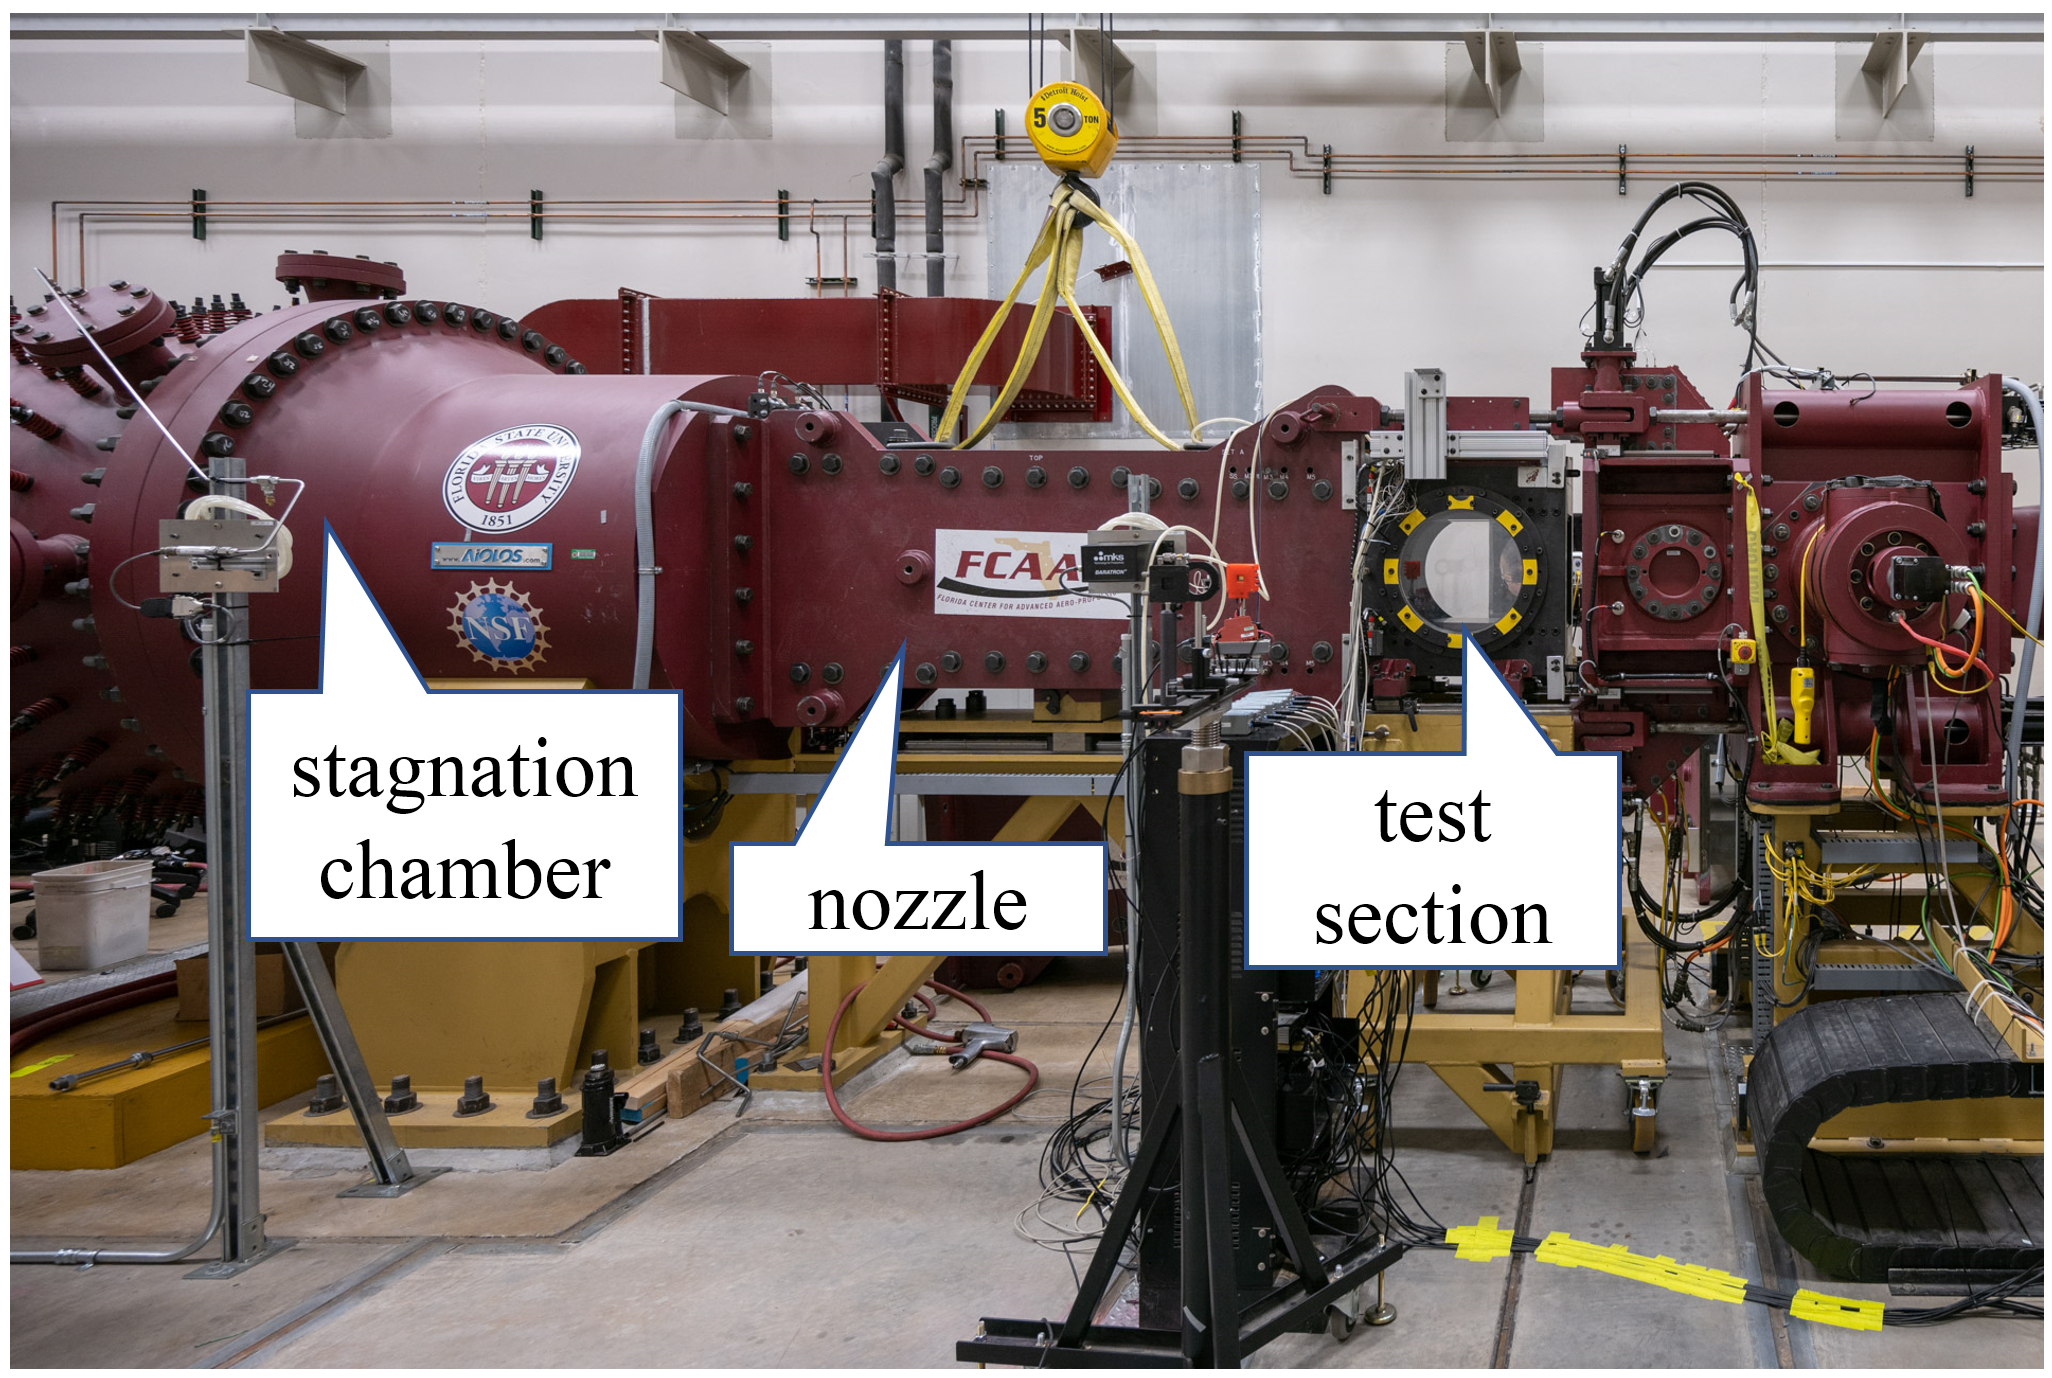
\includegraphics[width=0.7\linewidth]{./figures/fsu/PSWT.PNG}
    \caption{Polysonic wind tunnel}
    \label{fig:PSWT}
\end{figure}

\subsection{Test geometry and PIV setup}
The objective of the current set of experiments was to study shock-shock interactions over a range of Mach numbers and shock strengths. For this purpose, a set of wedge shock generators produces leading edge deflections of $5, 10,$ and $15^\circ$. The shock generators have a spanwise width of 0.14 m, which was a compromise between maintaining 2D flow on the tunnel centerline and keeping flow blockage low. To limit spanwise edge effects, the shock generators are mounted on diamond cross-section struts from the test section ceiling and floor, as shown in \ref{fig:PIVsetup}.\par

To allow PIV measurements in a vertical streamwise plane between the shock generators, a laser sheet was introduced through a window installed in the top test section plug downstream of the top strut. The laser used was an Evergreen EVG-200 200mJ per pulse Nd:YAG laser operated at a 7.23 Hz repetition rate and an inter-pulse spacing of 0.8, 1.0, and 0.7 $\mu \text{s}$ at Mach 2, 3, and 4, respectively. Planar PIV imaging was captured through the side window using two Lavision Imager Pro X cameras. Camera 1 was positioned to provide a view of the entire shock generator flow field, while Camera 2 was fitted to zoom in on the shock-shock interaction. Both cameras were repositioned accordingly as the location of the interaction moved throughout the length of the test section, given the changing shock strength and Mach number. At Mach 2, Camera 1 (wide) used a 50mm lens with a 1.4x teleconverter, and Camera 2 (zoomed in) used a 135mm lens with a 1.4x teleconverter. For Mach 3, the lenses were 135mm and 180mm, respectively, without teleconverters. Finally, at Mach 4 the lenses chosen were 50mm without teleconverter for Camera 1 and 180 mm lens with a 1.4x teleconverter for Camera 2.

\begin{figure}[ht!]
    \centering
    \includegraphics[width=0.7\linewidth]{./figures/fsu/PIVsetup.PNG}
    \caption{Test section side view showing shock generators on struts as well as the PIV laser sheet optics on top of the test section.}
    \label{fig:PIVsetup}
\end{figure}

\subsection{Seeding setup}
For this set of PIV tests, seeding was provided by a Wright nebulizer installed in a flanged pressure vessel as shown in \ref{fig:seedsystem}. The pressure vessel was filled above the nebulizer with Rosco Fog Fluid, a commercial fog generator fluid also used in low-pressure, heat-based fog generators, prior to testing. This is a viscous liquid consisting of various glycols in a water solution with a density of 1055-1075 kg/m\textsuperscript{3}. The seeder is provided air from the same high-pressure system as the wind tunnel with a regulator allowing the pressure to be set before the start of each tunnel blowdown and a solenoid valve allowing seeding to be started and stopped remotely from the control room after the tunnel has been started and after the completion of PIV image acquisition, respectively. The seeder pressure must be set to overcome the stagnation pressure at each Mach number to ensure good seeding. Here, the regulator outlet pressures were set at 0.55, 0.69, and 1.38 MPa for Mach 2, 3, and 4, respectively. At Mach 4, the seeding pressure was limited by the pressure rating of the seeder pressure vessel, and seeding was found to be less dense and consistent compared to the lower Mach numbers. Downstream of the nebulizer, the seed stream is fed into the wind tunnel stagnation chamber downstream of the flow conditioning meshes but upstream of the convergent section leading into the nozzle. The tunnel has two flanged ports, one on top and one on the bottom, which can be used to install a vertical seeder pipe with an outer diameter of 32 mm and an inner diameter of 27 mm. Two different pipes are available: a half-length one that utilizes a single port for seeding close to either the ceiling or the floor of the wind tunnel and a full-length one that provides seeding in the center of the test section. In this setup, which was used in the present set of tests, five 3.2-mm diameter holes facing upstream in the stagnation chamber are drilled into the vertical seed pipe to deliver the air-seed mixture into the chamber and ensure good mixing before it is convected into the test section. This arrangement, as well as the approximate 6 m of hose connecting the seeder to the seed pipe, likely has an impact on the delivered seed particle distribution as larger particles will tend to settle on walls and in bends as they are transported by low-velocity air to the stagnation chamber.
% FSU: Please add information about the setup. I can edit as needed. Thanks!

\begin{figure}[ht!]
        \centering
    \begin{subfigure}{0.35\linewidth}
        \centering
        \includegraphics[width=\linewidth]{./figures/fsu/Seeder_a.PNG}
        \caption{Wright nebulizer assembly removed from pressure vessel}
        \label{fig:wrightneb}
    \end{subfigure}%
    \begin{subfigure}{0.35\linewidth}
        \centering
        \includegraphics[width=\linewidth]{./figures/fsu/Seeder_b.PNG}
        \caption{Seeder shown with air supply line and outlet connected to top port on tunnel stagnation chamber}
        \label{fig:seedcon}
    \end{subfigure}
    \caption{Seeding system used for PIV measurements in the Polysonic Wind Tunnel}
    \label{fig:seedsystem}
\end{figure}
\subsection{PIV processing}

\section{Particle size distribution analysis}
% One of the reasons this is important is because we need to understand how much of an effect on particle distribution we are getting from coalesence/agglomeration
In this section, different particle distributions are explored to understand the variation of particle diameter on response times under similar conditions. This helps to understand the effect of particle coalescence, agglomeration, or breakup that occurs as these particles pass through an oblique shock. These particle distributions were tracked through an oblique shock using the Loth drag model and the Lagrangian Particle Tracking algorithm explored in the previous sections. The velocity of the particles past the shock was captured to perform a PIV-comparable response analysis. In addition, a novel methodology has been explored to estimate the particle size distribution. For this analysis, an oblique shock flow field generated at Mach 1.5 and a deflection angle of $10^\circ$ is used. This flow field is representative of most of the supersonic experiments conducted.\par
% \begin{enumerate}
%     \item A weak oblique shock generated at Mach 1.5 and a deflection angle of $10^\circ$
%     \item A weak oblique shock generated at Mach 5.0 and a deflection angle of $30^\circ$
% \end{enumerate}

% types of the distributions used % talk about the right skewness in data by plotting z-score
Two different types of distribution were tested to understand the effect of variance in particle diameter on response times in a given oblique shock. They are as follows:
\begin{enumerate}
    \item Gaussian distribution with a mean of 1940nm and a standard deviation of 250nm, shown in Fig. \ref{fig:gaussian_dia}
    \item Skew normal distribution with a shape parameter of 4, which is chosen to produce negative skewness. The location parameter, which describes the location of the skewness, is set to 1940nm. The scale parameter, which is similar to the standard deviation in a normal distribution, is set to 250nm. This produces a mean of $1749\text{nm}$. This data is shown in Fig. \ref{fig:skewnorm_dia}
\end{enumerate}

\begin{figure}[ht!]
    \begin{subfigure}{0.5\linewidth}
        \centering
        \includesvg[width=\linewidth]{./figures/polydisperse/gaussian_diameter}
        \caption{Gaussian distribution}
        \label{fig:gaussian_dia}
    \end{subfigure}%
    \begin{subfigure}{0.5\linewidth}
        \centering
        \includesvg[width=\linewidth]{./figures/polydisperse/skewnorm_diameter}
        \caption{Skew normal distribution}
        \label{fig:skewnorm_dia}
    \end{subfigure}
    \caption{Diameter distributions used to test the variance in particle response times}
    \label{fig:dia_distributions}
\end{figure}


The statistics were chosen from a theoretical standpoint and are not representative of any known particle diameter distributions used in the experiments. The mean particle size is chosen from the work of Williams et al. \cite{williams2015}. The tests were carried out similarly to the analysis of Mitchell et al. \cite{mitchell2011}, who used log-normal distributions in their study. These were shown to be the most prominent distributions in the wake of the particle generators shown by Kahler et al. \cite{kahler2002}.\par

In the current analysis, a total of 15000 particles were used to compute the distributions described. These particles were tracked using the LPT code, which was validated in the previous section. The z-statistics were calculated for both the diameter and response time distributions to compare the variance. This study helps to determine whether the response time distribution produced from a Gaussian particle diameter distribution is normal. This z-statistic data for both diameters and response times is plotted in Fig. \ref{fig:z_diavstime_1p5}. The data show that the response times are positively skewed (a type of distribution in which most values are clustered around the left tail of the distribution, while the right tail is longer) compared to the diameter, regardless of the type of underlying distribution for diameters. The amount of skewness is proportional to the variance in the diameter distribution. These results, coupled with our understanding of the importance of particle diameter from the previous section, suggest that to achieve a lower level of uncertainty related to tracer particle presence, it is important to consider the polydispersity of the particles and not just the mean particle diameter. This is particularly true if the variation in particle diameter is high, which can be attributed to the clustering or breakup of particles, depending on the flow properties.\par

\begin{figure}[ht!]
    \begin{subfigure}{0.5\linewidth}
        \centering
        \includesvg[width=\linewidth]{./figures/polydisperse/gaussian_zscore_comparison}
        \caption{Gaussian distribution}
        \label{fig:gaussian_zscore}
    \end{subfigure}%
    \begin{subfigure}{0.5\linewidth}
        \centering
        \includesvg[width=\linewidth]{./figures/polydisperse/skewnorm_zscore_comparison}
        \caption{Skew normal distribution}
        \label{fig:skewnorm_zscore}
    \end{subfigure}
    \caption{Comparing z-scores of response times to particle diameters for Mach 1.5 case}
    \label{fig:z_diavstime_1p5}
\end{figure}

In addition, the normalized shock velocity to the shock normal distance plots for both distributions are shown in Fig. \ref{fig:response_plots_distributions}. The data is fitted to a curve using Eq. \ref{eq:distance_equation}, recreating the PIV particle response analysis. Note that this assumption is based on the uncertainty from the imaging and analysis phase of PIV being negligible. This yielded a particle diameter of $2031\text{nm}$ and a response time of $ 6.62\mu\text{s}$ for the data obtained from the Gaussian distribution. These values are within 5\% of the values specified for the mean of the distribution. This is due to the cutoff point in the data used to replicate the process in PIV. For the skew-normal distribution, the curve fit analysis produced a particle diameter of $1822\text{nm}$ and a response time of $5.63\mu \text{s}$ versus a mean of $1749 \text{nm}$ for the original distribution. This is about 4\% deviation from the mean. This variation suggests that fitting a curve does not necessarily yield the diameter that best represents the original distribution, as indicated by the difference in mean estimates. It also does not provide information about the variation in particle diameters.\par

\begin{figure}[ht!]
    \begin{subfigure}{0.5\linewidth}
        \centering
        \includegraphics[width=\linewidth]{./figures/polydisperse/size_estimate_gaussian_m1p5_def10}
        \caption{Gaussian distribution}
        \label{fig:size_estimate_gaussian}
    \end{subfigure}%
    \begin{subfigure}{0.5\linewidth}
        \centering
        \includegraphics[width=\linewidth]{./figures/polydisperse/size_estimate_skewnorm_m1p5_def10}
        \caption{Skew normal distribution}
        \label{fig:size_estimate_skewnorm}
    \end{subfigure}
    \caption{Particle size estimate using the traditional curve fitting for Mach 1.5 case}
    \label{fig:response_plots_distributions}
\end{figure}


\section{Predictive modeling of particle size distribution}
% propose new analysis by stating how can we predict the underlying distribution and why it is relevant
Here, we propose a new analysis to predict the particle distribution using the existing data from particle response analysis. This can be used during any oblique shock-based particle response analysis to understand the underlying distribution captured in PIV. Note that the distribution picked up by the camera sensors in PIV typically has a lower cutoff due to the amount of light scattering. This is further discussed by Raffel et al. \cite{raffel2018}, who suggested that ideally, the ratio of particle diameter to laser wavelength should be greater than one to get enough scattering.\par


In analyzing the particle response to an oblique shock, the velocity field is obtained using the images generated from PIV. The velocity field can be tagged, and the velocity across a region of interest can be plotted to obtain exponential decay plots similar to Fig. \ref{fig:ragni_decay_solution}. This is a common way to estimate the mean particle diameter and has been observed in the work of Urban et al. \cite{urban2001} and Williams et al. \cite{williams2015}. Estimating the particle size distribution has implications for understanding the clusters or break-up of these particles in such flows, which in turn can help obtain accurate uncertainty bounds for the velocity field and turbulence statistics obtained from PIV. This can also help calibrate the experiment if the diameter variance is too high in the flow. The following steps can be used to estimate the particle distribution to an extent:
\begin{enumerate}
    \item \textbf{Data segmentation:} Divide the data into buckets using a range of response times and Eq. \ref{eq:distance_equation}.
    \item \textbf{Curve fitting:} Fit ``n'' curves by performing stratified sampling along the shock normal distance, sampling n-times within each bucket proportional to the amount of data in that bucket.
    \item \textbf{Compute statistics:} Compute the response time and diameters corresponding to each fit.
    \item \textbf{Z-statistics computation:} Z-statistics are calculated to normalize the data and remove bias from varying sample sizes.
    \item \textbf{Estimate distribution:} The mean particle diameter obtained from a single curve fit can be used to obtain information about the underlying particle distribution being picked by the camera sensors.
\end{enumerate}


For example, consider the distributions presented earlier. The particles are traced using the LPT code. The data obtained are randomly sampled to replicate the PIV shock-normal plot as seen in Fig. \ref{fig:ragni_decay_solution}. The verification of the current method was performed using the data-centric paradigm. By keeping the flow conditions constant across the test cases and the algorithm constant, we vary only the particle distributions to assess how the code performs in predicting variations in particle diameter. The results obtained are presented in Fig. \ref{fig:gaussian_predicted_distributions} and Fig. \ref{fig:skewnorm_predicted_distributions} for the Gaussian and Skew normal distributions, respectively.\par

\begin{figure}[ht!]
    \begin{subfigure}{0.5\linewidth}
        \centering
        \includesvg[width=\linewidth]{./figures/polydisperse/gaussian_m1p5_def10_diameter_comparison}
        \caption{Diameter distribution comparison}
        \label{fig:gaussian_dia_comparison}
    \end{subfigure}%
    \begin{subfigure}{0.5\linewidth}
        \centering
        \includesvg[width=\linewidth]{./figures/polydisperse/gaussian_m1p5_def10_diameter_zscore_comparison}
        \caption{Z-score comparison}
        \label{fig:gaussian_dia_z_score}
    \end{subfigure}
    \caption{Predicted vs. original data for Gaussian particle distributions}
    \label{fig:gaussian_predicted_distributions}
\end{figure}

The data presented in Fig. \ref{fig:gaussian_dia_comparison} highlight the ability of the current method to predict the underlying distribution of particles accurately. The observed gaps in particle diameter are attributed to inherent randomness in the sampling process. This phenomenon is elucidated by the z-score plot shown in Fig. \ref{fig:gaussian_dia_z_score}. The number of particles in the predicted distribution is counted as the total number of fits performed. Since this validation is approached by the data-centric paradigm, the number of fits have been adjusted to accurately predict the distributions for both cases under consideration. These numbers may require some adjustments for an accurate representation of a different data set. The predicted mean and standard deviation are found to be $1960nm$ and $265nm$, respectively.\par

\begin{figure}[ht!]
    \begin{subfigure}{0.5\linewidth}
        \centering
        \includesvg[width=\linewidth]{./figures/polydisperse/skewnorm_m1p5_def10_diameter_comparison}
        \caption{Diameter distribution comparison}
        \label{fig:skewnorm_dia_comparison}
    \end{subfigure}%
    \begin{subfigure}{0.5\linewidth}
        \centering
        \includesvg[width=\linewidth]{./figures/polydisperse/skewnorm_m1p5_def10_diameter_zscore_comparison}
        \caption{Z-score comparison}
        \label{fig:skewnorm_dia_z_score}
    \end{subfigure}
    \caption{Predicted vs. original data for Skew-normal particle distributions}
    \label{fig:skewnorm_predicted_distributions}
\end{figure}

The prediction for the skew-normal distribution is also performed using the same parameters used for the Gaussian data. The data in Fig. \ref{fig:skewnorm_predicted_distributions} show that the current method accurately predicts the skewness of the distribution. For the fitted data, the shape parameter was calculated to be 3.60, the location is $1920nm$, and the scale parameter is $217nm$. These parameters show that the fitted data are quantitatively compliant with the provided skew-normal distribution.\par

The analysis presented in this section underscores the critical importance of understanding particle size distributions in predicting response times within oblique shock environments. Using Gaussian and skew-normal distributions, the study reveals that the variance in particle diameter has a significant impact on response times, which are crucial for accurate PIV measurements. The method demonstrated here, using the Loth drag model and LPT code, along with curve fitting and z-statistics, provides a robust framework for predicting the underlying particle distributions. The findings indicate that even when particle distributions exhibit significant skewness or variance, the current methodology can accurately capture these characteristics, ensuring that the mean and standard deviation of the predicted data align closely with the original distributions. This highlights the need to consider polydispersity in particle distributions to quantify uncertainty in experimental outcomes, especially in high-variance scenarios influenced by particle coalescence, agglomeration, or breakup. Such insights are vital for refining PIV experiments and enhancing the accuracy of flow diagnostics in supersonic and other complex flow regimes.\par


\section{Particle size distribution in a shock interaction experiment}
It is established in several works (Urban and Mungal \cite{urban2001}, Mitchell et al. \cite{mitchell2011}, and Williams et al. \cite{williams2015}) that the particle properties during a PIV run vary in comparison to the distribution obtained from the seeder. This is due to two factors: agglomeration/breakup, which affects the mean particle size and density, and the ability of particles to reflect light that is captured by the camera sensor, which skews the particle distribution observed in the images. These factors make it essential to understand the particle distribution picked up by the PIV imaging system, which can help estimate the range of Stokes number. This helps define uncertainty bounds due to tracer particles in a PIV experiment. The size distribution analysis described in the previous section is extended to the shock interaction PIV experiments in this section.\par

Two different shock interaction cases were studied for the current study. The first case involved a Mach 2.0 flow with shock generators configured at deflection angles of $5^\circ$ and $5^\circ$, while the second configuration utilized deflection angles of $10^\circ$ and $10^\circ$. The corresponding shadowgraphs for these configurations are presented in Fig. \ref{fig:shadowgraph_shock_interaction}, illustrating the resultant shock structures and interaction regions. These visualizations provide critical insights into the flow characteristics, including the shock wave formations, interaction patterns, and potential separation zones.\par

The comparison of these cases underscores the influence of deflection angles on the complexity and intensity of shock interactions. The incident shocks formed from the deflectors are isolated to estimate the particle distribution. This approach minimizes interference from other flow features that happen in the post-interaction region, ensuring a more accurate assessment within the designated region.\par

\begin{figure}[ht!]
    \begin{subfigure}{0.5\linewidth}
        \centering
        \includegraphics[width=\linewidth]{./figures/fsu/Mach2_5_5.png}
        \caption{Mach2 - $5^\circ$ and $5^\circ$}
        \label{fig:shadowgraph_shock_interaction1}
    \end{subfigure}%
    \begin{subfigure}{0.5\linewidth}
        \centering
        \includegraphics[width=\linewidth]{./figures/fsu/Mach2_10_10.png}
        \caption{Mach2 - $10^\circ$ and $10^\circ$}
        \label{fig:shadowgraph_shock_interaction2}
    \end{subfigure}
    \caption{Shadowgraphs of shock interaction cases under study}
    \label{fig:shadowgraph_shock_interaction}
\end{figure}

The data obtained from the PIV experiment is processed using DaVis 11.2 software. The average velocity contours are obtained with multiple interrogation windows with 75\% overlap. This data is normalized using Eq. \ref{eq:exponential_decay}, and the data at each node in the grid is plotted against the x-direction. To establish a consistent reference, the incident shock location was set to zero by identifying the velocity drop characteristic of the shock. The data was further refined to isolate information from the incident shock region. This filtering was achieved by utilizing the post-shock velocity predicted from isentropic oblique shock relations. The resulting data is presented in Fig. \ref{fig:shock_location_plot}. The observed spread in the data is attributed to the particle size and the interrogation window size, which was 64×64 for the current case.\par

\begin{figure}[ht!]
    \begin{subfigure}{0.5\linewidth}
        \centering
        \includegraphics[width=\linewidth]{./figures/fsu/M2_5_5_64x64_normalized.png}
        \caption{Mach2 - $5^\circ$ and $5^\circ$}
        \label{fig:shock_location_plot1}
    \end{subfigure}%
    \begin{subfigure}{0.5\linewidth}
        \centering
        \includegraphics[width=\linewidth]{./figures/fsu/M2_10_10_64x64_normalized.png}
        \caption{Mach2 - $10^\circ$ and $10^\circ$}
        \label{fig:shock_location_plot2}
    \end{subfigure}
    \caption{Shock location adjusted normalized velocity}
    \label{fig:shock_location_plot}
\end{figure}

The data from Fig. \ref{fig:shock_location_plot} is further reduced by removing any velocity below the post-shock velocity. This helps isolate the data relevant to the oblique shock. An uncertainty bound of 0.5\% was incorporated during this data reduction process to account for uncertainties inherent in the image analysis. For instance, in the case of a Mach 2.0 flow with a deflection angle of $5^\circ$, the pre-shock velocity was set to $510m/s$, and the post-shock velocity was determined to be $480m/s$. This approach ensures a robust analysis of the shock region while mitigating the impact of measurement uncertainties.\par

The nominal diameter and density of the particle were computed using the two-equation approach presented in section \ref{sec:lpt}. The diameter and density of the particles were estimated to be $0.808 \mu m$ and $1408 kg/m^3$, respectively.\par

Understanding that the current particle sizing analysis depends on the uncertainties arising throughout the PIV experiment is essential. Lazar et al. \cite{lazar2010} showed that most uncertainty arises from particle dynamics and cross-correlation performed in PIV for a supersonic crossflow case. Since isolating the uncertainty generated from the analysis aspect is currently not possible, a sensitivity analysis is performed to understand the particle size distribution. The methodology described in the previous section is applied to the isolated data present in Fig. \ref{fig:shock_location_plot}.\par

% TODO: We might need to add the two-equation two-variable (diameter and density) problem.

% 
\subsection{Mach 2.0 $5^\circ/5^\circ$}
The results obtained for different interrogation window sizes for Mach 2.0 $5^\circ/5^\circ$ case are presented in Fig. \ref{fig:dia_distribution_5-5}. The histograms in each subplot represent the distribution of particle diameters in microns under different spatial resolutions. These distributions are multimodal, indicating the presence of distinct particle groups being detected during the experiment. This can happen for several reasons, such as agglomeration, breakup, or heterogeneous particle generation. The spatial resolution significantly influences the density peaks and smoothness of the distributions. For example, the highest resolution case (0.087 mm) captures finer details of the size distribution, showing sharper and more frequent peaks compared to the coarsest (0.465 mm) resolution case, which could suggest a loss of information relevant to particle sizes resulting from the analysis. This implies that the larger particles dominate the signal strength in coarser resolutions, and broader distributions average out the particle characteristics.\par

\begin{figure}[ht!]
    \centering
    \includegraphics[width=\linewidth]{figures/fsu/diameter_distribution_5-5.png}
    \caption{Particle diameter distributions for Mach 2.0 $5^\circ/5^\circ$ case at different spatial resolutions}
    \label{fig:dia_distribution_5-5}
\end{figure}

The particle size analysis from the PIV data reveals that the mean particle size remains consistent across all spatial resolutions, ranging between $0.8 - 1.0 \mu m$. At finer spatial resolutions (e.g., 0.087 mm), the particle size distribution appears almost uniform, showcasing the ability of the PIV system to resolve particles more accurately. This uniformity is crucial for PIV cross-correlation algorithms, as it ensures a balanced contribution from all particle sizes, leading to more reliable and accurate velocity field estimations. In contrast, coarser spatial resolutions (e.g., 0.465 mm) exhibit skewed distributions, with larger particles dominating due to reduced detection of smaller particles. This skewness can introduce biases in velocity estimations, particularly in regions of high gradients, such as oblique shocks, where particle inertia effects are significant. These findings highlight the importance of finer spatial resolutions in preserving the uniform distribution necessary for optimal algorithm performance.\par

% Particle relaxation times and stokes number
% -- Multimodal; Stokes number can be computed using the smallest time scale measurement possible

% flow characteristic time is spatial resolution / max. velocity

\begin{figure}[ht!]
    \centering
    \includegraphics[width=\linewidth]{figures/fsu/stokes_number_distribution_5-5.png}
    \caption{Stokes number distributions for Mach 2.0 $5^\circ/5^\circ$ case at different spatial resolutions}
    \label{fig:stokes_distribution_5-5}
\end{figure}

The Stokes number ($St$) distributions are analyzed to quantify uncertainties and establish reliable bounds for the measurement setup. The characteristic flow time is chosen based on a macroscopic geometric scale relevant to the shock interaction. Specifically, the throat distance between the shock generators, $L_f = 88\,\mathrm{mm}$, is used as the characteristic length for all configurations. The flow characteristic time in Eq.~\ref{eq:stokes_number} is calculated using the free-stream velocity. The resulting Stokes number reflects the dynamics at the scale of the global shock interaction features. It is important to note that this Stokes number does not account for microscopic flow features, such as shock wave thickness or fine-scale interaction regions.
\par

Figure \ref{fig:stokes_distribution_5-5} shows that the Stokes number is well below one. This indicates that the particles effectively track flow dynamics within acceptable limits of particle inertia effects. The Stokes number distributions exhibit a noticeable rightward skew compared to the particle size distributions. This observation highlights the non-linear nature of the drag force acting on the particles, which governs their motion and leads to this distinct skew. This behavior is consistent with the findings of our numerical analysis in the previous section.\par

Figure \ref{fig:stokes_distribution_5-5} further underscores notable trends in Stokes number distributions across spatial resolutions. As spatial resolution coarsens, the mean Stokes number increases from 0.025 at 0.087 mm to 0.038 at 0.465 mm. This trend reflects a reduction in particle inertia effects at finer resolutions, allowing particles to respond better to flow features due to the constraints imposed by a finer computational grid. The results confirm that higher spatial resolutions are critical for accurately capturing small-scale flow features, particularly in complex flow scenarios involving shocks or vortices.\par

The adherence to St < 0.05 across all cases validates the robustness of the setup within recommended bounds. This finding is essential for applications where particle inertia effects could significantly alter the flow-field representation. Spatial resolution directly impacts uncertainty quantification, with finer resolutions providing greater certainty. Therefore, the choice of resolution must carefully balance computational cost against the need for accuracy, particularly in studies where precision in resolving critical flow features is paramount.\par

% \begin{figure}[ht!]
%     \centering
%     \includegraphics[width=\linewidth]{figures/fsu/response_time_distribution_5-5.png}
%     \caption{Particle response distributions for Mach 2.0 $5^\circ/5^\circ$ case at different spatial resolutions}
%     \label{fig:relaxation_time_5-5}
% \end{figure}


% Finally, the laser pulse time is about $0.8 \mu s$. This is well below the range of relaxation time observed for particles. This is shown in Fig. \ref{fig:relaxation_time_5-5}.

\subsection{Mach 2.0 $10^\circ/10^\circ$}
The results obtained for different interrogation window sizes for the Mach 2.0 $10^\circ/10^\circ$ case are presented in Fig. \ref{fig:dia_distribution_10-10}. The histograms in each subplot represent the distribution of particle diameters in microns under different spatial resolutions. Similar to the $5^\circ/5^\circ$ case, these distributions are multimodal, indicating distinct particle groups detected during the experiment. The multimodality is particularly pronounced at finer resolutions (first three subplots), where the higher spatial fidelity enables the clear identification of particle clusters. However, at coarser resolutions, the blending of these particle groups becomes more apparent, likely due to the reduced ability to distinguish smaller particles and clusters.\par

Compared to the $5^\circ/5^\circ$ case, the increased multimodality observed in the $10^\circ/10^\circ$ case may indicate stronger flow disturbances or unique clustering effects caused by the larger deflection angles. This highlights how the flow field itself can significantly influence particle size distributions and the degree of clustering.\par

The distributions taper off at larger diameters, with particle diameters exceeding one micron being nearly negligible. However, these larger diameters become more noticeable as the resolution coarsens. This trend likely arises from a loss of information in particle sizing at coarser resolutions, where the inability to resolve finer details leads to the apparent detection of larger particle sizes. These results underscore the significance of spatial resolution in determining particle size.\par



\begin{figure}[ht!]
    \centering
    \includegraphics[width=\linewidth]{figures/fsu/diameter_distribution_10-10.png}
    \caption{Particle diameter distributions for Mach 2.0 $10^\circ/10^\circ$ case at different spatial resolutions}
    \label{fig:dia_distribution_10-10}
\end{figure}

Like the $5^\circ/5^\circ$ case, the Stokes number, shown in Fig. \ref{fig:stokes_distribution_10-10}, remains well below the recommended threshold for studying supersonic flows. While a stronger shock and larger mean particle diameter would typically result in a higher Stokes number, the distribution in this case exhibits significant right skewness, leading to a Stokes number that is comparable to the $5^\circ/5^\circ$ case. This behavior may be attributed to the breakup of liquid particles as they traverse the shock interface, resulting in smaller particle sizes that reduce the effective Stokes number. The Stokes number is also clustered around two significant peaks, similar to the diameter distribution. However, the effect of these peaks is more comparable, indicating the non-linearity of the Stokes number in relation to diameter.\par

\begin{figure}[ht!]
    \centering
    \includegraphics[width=\linewidth]{figures/fsu/stokes_number_distribution_10-10.png}
    \caption{Stokes number distributions for Mach 2.0 $10^\circ/10^\circ$ case at different spatial resolutions}
    \label{fig:stokes_distribution_10-10}
\end{figure}

These results highlight the critical role of spatial resolution and interrogation window size in accurately resolving particle dynamics. Understanding these dynamics helps to bound uncertainty in velocity estimation from PIV accurately. For high-gradient flows, such as those involving shocks, finer resolutions are essential to accurately quantify biases introduced by particle inertia and ensure reliable velocity measurements.\par

% comments on the effects of temporal resolution

\section{Particle dynamics history analysis}
The particle sizes obtained were used to conduct a particle dynamics history analysis to better validate the CFD data obtained for the Mach 2 $10^\circ/10^\circ$ case. The CFD simulation was conducted using ANSYS 2021 R2.\par

The initial grid of the domain under study to start the simulation is shown in Fig. \ref{fig:fsu_initial_grid}. The grid is refined in the shock interaction region to have a maximum cell thickness of $0.1mm$, totaling 33,097 cells. An adaptive mesh refinement strategy was utilized to capture the shock interaction region. The refinement is set to split the grid up to 8 levels of refinement using a gradient adaptation approach with a factor of 0.5. This process yielded a grid size of approximately $10^{-5} m$ in the shock cells. This final grid is shown in Fig. \ref{fig:fsu_final_grid}\par

\begin{figure}[ht!]
    \begin{subfigure}{0.5\linewidth}
        \centering
        \includegraphics[width=\linewidth]{phd_dissertation/figures/fsu/pdh/original_mesh_logo_removed.png}
        \caption{Initial grid}
        \label{fig:fsu_initial_grid}
    \end{subfigure}%
    \begin{subfigure}{0.5\linewidth}
        \centering
        \includegraphics[width=\linewidth]{phd_dissertation/figures/fsu/pdh/adapted_mesh_logo_removed.png}
        \caption{Final grid}
        \label{fig:fsu_final_grid}
    \end{subfigure}
    \caption{Initial and final grids to capture shock interaction for Mach 2 $10^\circ/10^\circ$}
    \label{fig:fsu_grids}
\end{figure}

The Reynolds-averaged Navier-Stokes (RANS) equations are solved using the \(k\)-\(\omega\) turbulence model, where \(k\) is the turbulence kinetic energy and \(\omega\) is the specific rate of dissipation of turbulence. This model is chosen due to its robustness in capturing regions with adverse pressure gradients.

In the Fluent solver, the operating pressure is set to 0~Pa. The boundary conditions are defined as follows:

\begin{itemize}
    \item \textbf{Inlet}: Set to pressure inlet. The gauge total pressure of 280,000~Pa, supersonic/initial gauge pressure of 35,785.27~Pa, and total temperature of 291.25~K.
    \item \textbf{Outlet}: Set to pressure outlet. The gauge pressure was 35,785.27~Pa.
    \item \textbf{Domain boundaries}: Set to far-field pressure conditions with a gauge pressure of 35,785.27~Pa.
    \item \textbf{Wedges}: The walls of the wedges are set to no-slip.
\end{itemize}

The velocity profile for the converged CFD data is shown in Fig.~\ref{fig:u_cfd}, while the corresponding PIV data is presented in Fig.~\ref{fig:u_piv}. The velocity contours are normalized by the free-stream velocity of 510~m/s. 

The PIV data is well-resolved, effectively capturing the incident shocks and their interaction region, which is the primary focus of this study. The regions with zero velocity in the PIV results are a consequence of experimental setup limitations, where optical constraints prevent data acquisition in those areas. The CFD data exhibits finer resolution due to the higher grid refinement, allowing for a more detailed representation of the flow structures. This data is further analyzed by tracking particles using the LPT code from Chapter \ref{ch:lpt}


\begin{figure}[ht!]
    \begin{subfigure}{0.5\linewidth}
        \centering
        \includegraphics[width=\linewidth]{phd_dissertation/figures/fsu/pdh/u_contour_normalized.png}
        \caption{CFD}
        \label{fig:u_cfd}
    \end{subfigure}%
    \begin{subfigure}{0.5\linewidth}
        \centering
        \includegraphics[width=\linewidth]{phd_dissertation/figures/fsu/pdh/mach2_10-10_velocity_contour.png}
        \caption{PIV}
        \label{fig:u_piv}
    \end{subfigure}
    \caption{Normalized velocity contours for shock interaction case, Mach 2 $10^\circ/10^\circ$}
    \label{fig:shock_interaction_u_contours}
\end{figure}

Further analysis was conducted by extracting velocity profiles at three different locations based on the particle relaxation distance. These profiles are shown in Fig. \ref{fig:fsu_pdh_study}. A spatial bias is applied by interpolating the numerical data onto an equidistant grid of size 0.086mm to all the data except for the ``CFD data -- raw", which is the data obtained from the CFD simulation and has finer resolution. Particles of significance (average of $0.8 \mu m$, peak size $1.2 \mu m$, and maximum size $1.5 \mu m$) found during the size distribution analysis were used to perform this analysis.\par

\begin{figure}[ht!]
    \centering
    \begin{subfigure}{0.5\linewidth}
        \centering
        \includegraphics[width=\linewidth]{phd_dissertation/figures/fsu/pdh/shock_interaction_spatial_bias_0p5mm.png}
        \caption{Incomplete relaxation}
        \label{fig:0p5mm}
    \end{subfigure}\\
    \begin{subfigure}{0.5\linewidth}
        \centering
        \includegraphics[width=\linewidth]{phd_dissertation/figures/fsu/pdh/shock_interaction_spatial_bias_1mm.png}
        \caption{Moderate relaxation}
        \label{fig:1mm}
    \end{subfigure}%
    \begin{subfigure}{0.5\linewidth}
        \centering
        \includegraphics[width=\linewidth]{phd_dissertation/figures/fsu/pdh/shock_interaction_spatial_bias_5mm.png}
        \caption{Complete relaxation}
        \label{fig:5mm}
    \end{subfigure}
    \caption{PDH study in shock interaction distance vs. normalized velocity}
    \label{fig:fsu_pdh_study}
\end{figure}

At the $y = 0.5\ \mathrm{mm}$ location, none of the particle sizes tested relaxed to the post-shock velocity before encountering the second shock. This region, where the shocks are closely spaced, clearly exhibits the particle dynamics history (PDH) effect. Table \ref{tab:fsu_pdh_error} presents the L2-norm error between numerical datasets and PIV measurements within this inter-shock region. The error trends correlate strongly with particle inertia bias, indicating that incomplete velocity relaxation contributes to significant deviation between CFD and PIV data. This interpretation helps quantify the uncertainty introduced by particle inertia and provides a means to validate the numerical models more rigorously. The improvement in error between CFD and PIV data when accounted for PDH using different particle sizes is presented in Table \ref{tab:fsu_pdh_error_improvement}. At this location, the highest improvement is at around 85\%, indicating a significant PDH effect when there is incomplete particle relaxation.

\begin{table}[ht!]
\centering
\begin{tabular}{|cccc|}
\hline
\multicolumn{4}{|c|}{L2-norm error of data to PIV} \\ \hline
\multicolumn{1}{|c|}{Data} & \multicolumn{1}{c|}{Incomplete relaxation} & \multicolumn{1}{c|}{Moderate relaxation} & Complete relaxation \\ \hline
\multicolumn{1}{|c|}{CFD} & \multicolumn{1}{c|}{6.95\%} & \multicolumn{1}{c|}{6.13\%} & 3.25\% \\ \hline
\multicolumn{1}{|c|}{$0.8 \mu m$} & \multicolumn{1}{c|}{4.39\%} & \multicolumn{1}{c|}{4.00\%} & 1.83\% \\ \hline
\multicolumn{1}{|c|}{$1.2 \mu m$} & \multicolumn{1}{c|}{1.76\%} & \multicolumn{1}{c|}{1.49\%} & \textbf{0.80\%} \\ \hline
\multicolumn{1}{|c|}{$1.5 \mu m$} & \multicolumn{1}{c|}{\textbf{1.04\%}} & \multicolumn{1}{c|}{\textbf{0.97\%}} & 1.00\% \\ \hline
\end{tabular}
\caption{The error between PIV and the numerical data}
\label{tab:fsu_pdh_error}
\end{table}

At the $y = 1\ \mathrm{mm}$ location, the smallest particle size tested relaxed to the post-shock velocity shortly after the first shock. The medium-sized particles agreed with the velocity profile predicted by PIV in this region. After the second shock, the largest particle size tested aligned better with PIV results beyond the $x = 4\ \mathrm{mm}$ mark. The L2-norm error was similar for both medium and large particle sizes, indicating a breakup behavior that requires further study using particle-particle interaction models or in situ experiments. The improvement in error at this location is at 84.18\%, which was obtained using the largest particle size tested.

At the $y = 5\ \mathrm{mm}$ location, the PIV data aligned best with the medium particle size tested. This is evident from the low error compared to other particle sizes in the region. Compared to the other locations, the low error found at this location can be attributed to the full particle relaxation between shocks. Due to the full relaxation, the error improvement is also low at this location. These insights highlight that the averaging in PIV data carries a location-dependent particle inertia bias, which is influenced by the flow interaction spacing. This analysis helps in the better interpretation of PIV data. A detailed analysis incorporating the particle size distributions throughout the flow field would improve the agreement with experimental data.


\begin{table}[ht!]
\centering
\begin{tabular}{|cccc|}
\hline
\multicolumn{4}{|c|}{Percent improvement in error} \\ \hline
\multicolumn{1}{|c|}{Data} & \multicolumn{1}{c|}{Incomplete relaxation} & \multicolumn{1}{c|}{Moderate relaxation} & Complete relaxation \\ \hline
\multicolumn{1}{|c|}{$0.8 \mu m$} & \multicolumn{1}{c|}{36.83\%} & \multicolumn{1}{c|}{34.75\%} & 43.69\% \\ \hline
\multicolumn{1}{|c|}{$1.2 \mu m$} & \multicolumn{1}{c|}{74.67\%} & \multicolumn{1}{c|}{75.69\%} & \textbf{75.38\%} \\ \hline
\multicolumn{1}{|c|}{$1.5 \mu m$} & \multicolumn{1}{c|}{\textbf{85.03\%}} & \multicolumn{1}{c|}{\textbf{84.18\%}} & 69.23\% \\ \hline
\end{tabular}
\caption{The error improvement between PIV and CFD when accounted for PDH}
\label{tab:fsu_pdh_error_improvement}
\end{table}

\section{Conclusion}
% update conclusion based on what's going to be in the work
This numerical study of the response of particles in optical velocimetry experiments has yielded several significant findings and methodological advancements. The Loth and Tedeschi models were utilized due to their superior performance in accounting for inertial, compressibility, and rarefaction effects, thereby providing more accurate predictions of particle behavior. The particle response study, typically performed in supersonic PIV experiments to quantify the particle inertia bias, was explored in detail. The findings showed that the nominal size and density must be obtained through a two-equation model from which underlying distributions can be inferred. This study also acted as a validation for our in-house LPT code.\par

The investigation of particle size distributions reveals that response times are positively skewed compared to diameter distributions, emphasizing the importance of considering polydispersity in uncertainty quantification. For instance, a Gaussian distribution of particle diameters yielded a positively skewed distribution of response times, indicating a nonlinear relationship between particle size and response characteristics.\par

The proposed method for estimating underlying particle distributions from oblique shock response data offers a new tool for researchers to better understand and account for particle agglomeration and breakup in supersonic flows. This method successfully predicted the underlying distribution parameters with less than 1\% error for Gaussian distributions and accurately captured the skewness (shape parameter of 3.69 vs. 4.0) for skew-normal distributions.\par

These findings have significant implications for improving the accuracy of PIV measurements in complex flow environments. The updated distribution due to the effects of clustering or breakup can be captured using the novel proposed method. This helps in understanding the particle distribution in PIV and calibrates the experiment to reduce uncertainty caused by variations in particle sizes. The uncertainty related to the particle dynamics can also be accurately quantified if the variation in the particle distribution is understood.\par

Furthermore, the analysis of shock interaction experiments showcases the sensitivity of particle response characteristics to spatial resolution and interrogation window size. The shock interaction experiments reveal that the particle size is either nearly uniform or exhibits a clustering effect, depending on the specific case under study. The Stokes number for all these cases is well below the recommended Stokes number from the literature, highlighting the capability of the current experiments to provide accurate measurements. These findings underscore the importance of finer spatial resolutions in capturing accurate velocity fields, particularly in high-gradient flow regions like shocks.\par

A particle dynamics history analysis was conducted using the particle sizes found during the size distribution analysis. A RANS simulation was used to perform this analysis. A significant improvement in the error between CFD and PIV data was found, indicating the impact of PDH on PIV data. This analysis highlighted a methodology to validate CFD better with PIV data by incorporating accurate particle sizes, unlike most previous studies, where error reduction is achieved by increasing the Stokes number.

In summary, this work advances our understanding of particle dynamics in PIV experiments and introduces methodologies to address critical challenges related to particle size estimation and uncertainty quantification. The findings have direct implications for enhancing the reliability of PIV measurements in supersonic and other complex flow environments, paving the way for more accurate and insightful experimental fluid dynamics research.

Future research should focus on the experimental validation of the proposed distribution estimation method across a wide range of flows, as well as further investigation into the effects of particle dynamics history on measurement uncertainties under diverse flow conditions. Furthermore, extending this analysis to other types of optical velocimetry techniques could provide valuable information for the broader field of flow measurement.\par

